\documentclass{estilo}
\usepackage[spanish]{babel}
\usepackage{graphicx}
\usepackage{float}
\usepackage{amsmath}        % para los vectores columnas
\usepackage{amsfonts}       % para las negrita de pizarra
\usepackage{amssymb}        % para simbolos matematicos
\usepackage{hyperref}       % para utilizar referencias
\usepackage{multirow}       % para las tablas
\usepackage{dsfont}
\usepackage{listings}
\usepackage{xcolor}
\definecolor{codegreen}{rgb}{0,0.6,0}
\definecolor{codegray}{rgb}{0.5,0.5,0.5}
\definecolor{codepurple}{rgb}{0.58,0,0.82}
\definecolor{backcolour}{rgb}{0.95,0.95,0.92}
\lstdefinestyle{mystyle}{
    backgroundcolor=\color{backcolour},   
    commentstyle=\color{codegreen},
    keywordstyle=\color{magenta},
    numberstyle=\tiny\color{codegray},
    stringstyle=\color{codepurple},
    basicstyle=\ttfamily\footnotesize,
    breakatwhitespace=false,         
    breaklines=true,                 
    captionpos=b,                    
    keepspaces=true,                 
    numbers=left,                    
    numbersep=5pt,                  
    showspaces=false,                
    showstringspaces=false,
    showtabs=false,                  
    tabsize=2
}
\lstset{style=mystyle}

\usepackage{enumitem,multicol,setspace}
\newcounter{subenum}[enumi] % para las multicolumnas
\renewcommand{\thesubenum}{\arabic{subenum}}
\usepackage[nomessages]{fp}
\FPeval\thecolwidth{round(1/4:4)}% Specify number of columns -> column width
\newcommand{\newitem}[1]{%
  \refstepcounter{subenum}%
  \parbox{\dimexpr\thecolwidth\linewidth-.5\columnsep}{%
    \makebox[\labelwidth][r]{(\thesubenum)\hspace*{\labelsep}}%
    #1}\hfill%
}

\usepackage{scalerel,stackengine} % para el sombrero
\stackMath
\newcommand\rhat[1]{%
\savestack{\tmpbox}{\stretchto{%
  \scaleto{%
    \scalerel*[\widthof{\ensuremath{#1}}]{\kern-.6pt\bigwedge\kern-.6pt}%
    {\rule[-\textheight/2]{1ex}{\textheight}}%WIDTH-LIMITED BIG WEDGE
  }{\textheight}% 
}{0.5ex}}%
\stackon[1pt]{#1}{\tmpbox}%
}
\parskip 1ex

\usepackage{mathtools}      % floor y ceil
\DeclarePairedDelimiter\ceil{\lceil}{\rceil}
\DeclarePairedDelimiter\floor{\lfloor}{\rfloor} 

\usepackage[style=authoryear-comp]{biblatex}


\begin{document}
\maketitle

\justifying{}

\newpage
\justifying{
%\hypertarget{res}{\section*{Ejemplo de Resolución}}
\section{Análisis del problema}

\subsection{El problema}

El problema el cual vamos a resolver en este trabajo es el siguiente:


\setlength{\leftskip}{4em} % Apply left indentation for the entire paragraph
Trabajamos para la mafia de los amigos Amarilla Pérez y el Gringo Hinz. En estos momentos hay un problema: alguien les está robando dinero. No saben bien cómo, no saben exactamente cuándo, y por supuesto que no saben quién. Evidentemente quien lo está haciendo es muy hábil (probablemente haya aprendido de sus mentores).

La única información con la que contamos son $n$ transacciones sospechosas, de las que tenemos un timestamp aproximado. Es decir, tenemos n tiempos \(t_i\), con un posible error \(e_i\). Por lo tanto, sabemos que dichas transacciones fueron realizadas en el intervalo \([t_i - e_i; t_i + e_i]\).

Por medio de métodos de los cuales es mejor no estar al tanto, un interrogado dio el nombre de alguien que podría ser la rata. El Gringo nos pidió revisar las transacciones realizadas por dicha persona… en efecto, eran $n$ transacciones. Pero falta saber si, en efecto, condicen con los timestamps aproximados que habíamos obtenido previamente.

El Gringo nos dio la orden de implementar un algoritmo que determine si, en efecto, las transacciones coinciden. Amarilla Perez nos sugirió que nos apuremos, si es que no queremos ser nosotros los siguientes sospechosos.

\begin{itemize}
	\setlength{\leftskip}{3em} % Apply left indentation for the entire paragraph
	\item Hacer un análisis del problema, y proponer un algoritmo greedy que obtenga la solución al problema planteado: Dados los $n$ valores de los timestamps aproximados \(t_i\) y sus correspondientes errores \(e_i\), así como los timestamps de las $n$ operaciones \(s_i\) del sospechoso (pueden asumir que estos últimos vienen ordenados), indicar si el sospechoso es en efecto la rata y, si lo es, mostrar cuál timestamp coincide con cuál timestamp aproximado y error. Es importante notar que los intervalos de los timestamps aproximados pueden solaparse parcial o totalmente.
	\item Demostrar que el algoritmo planteado determina correctamente siempre si los timestamps del sospechoso corresponden a los intervalos sospechosos, o no. Es decir, si condicen, que encuentra la asignación, y si no condicen, que el algoritmo detecta esto, en todos los casos.
	\item Escribir el algoritmo planteado. Describir y justificar la complejidad de dicho algoritmo. Analizar si (y cómo) afecta la variabilidad de los valores de los diferentes valores a los tiempos del algoritmo planteado.
	\item Realizar ejemplos de ejecución para encontrar soluciones y corroborar lo encontrado. Adicionalmente, el curso proveerá con algunos casos particulares para que puedan usar de prueba.
	\item Hacer mediciones de tiempos para corroborar la complejidad teórica indicada. Esto, por supuesto, implica que deben generar sus sets de datos. Agregar los casos de prueba necesarios para dicha corroboración. Esta corroboración empírica debe realizarse confeccionando gráficos correspondientes, y utilizando la técnica de cuadrados mínimos.
	\item Agregar cualquier conclusión que les parezca relevante.
\end{itemize}

\setlength{\leftskip}{0em}


\subsection{Solución propuesta}

COMPLETAR...

AQUI DEBERIA ESTAR EL ANALISIS DEL PROBLEMA Y LA JUSTIFICACIÓN DE PORQUE FUNCIONA









\section{Algoritmo para asignar operaciones a intervalos}

\subsection{Código}


A continuación se muestra el código de la solución greedy del problema. 


\lstinputlisting[language=Python,firstline=8]{../src/moleFinder.py}

% Si queremos importar el código directo desde un archivo, podemos hacer lo siguiente: 

% \lstinputlisting[language=Python]{code/maximo_iterativo.py}

% Ventaja: evitamos copiar y pegar, y que si en un momento se modifique el algoritmo (reentrega, o la razón que fuere) no nos tengamos que acordar de esto más allá de compilar. 

% Desventaja: tenemos que asegurarnos de modularizar el código en archivos en función de cómo queremos mostrar el informe. Por otro lado, esto tiene especial sentido si estamos trabajando todo de forma local. Es decir, en el caso que no usemos Overleaf, porque sino implica tener que copiar el código de todas formas. 

% Mencionamos esta alternativa para que sepan que existe, ustedes definen cómo prefieren trabajar con esto. No nos interesa el código del informe, sólo el pdf resultante. 

\subsection{Análisis de complejidad}

La complejidad del algoritmo planteado posee dos partes identificables, el ordenamiento mediante MergeSort de los timestamp por tiempo de fin y la asignacion de las transacciones a un timestamp

Primero, hagamos un rapido analisis del ordenamiento MergeSort, este algoritmo divide el arreglo en subarreglos de la mitad de tamaño hasta llegar a un unico elemento, el cual se considera ordenado, luego combina los mismos de manera ordenada hasta llegar a nuestro arrreglo original ordenado en su totalidad. Si hablamos solo de temas de complejidad esta parte de nuestra respuesta tiene $\mathcal{O}\left(n \log n\right)$.

Por otro lado tenemos la parte principal del algoritmo, lo que busca es asignar cada transacción a un timestamp diferente. Consigue esto tomando y verificando dentro de que timestamps se encuentra y asociándolo al que termina antes, y esto se realiza por cada transacción. Por lo tanto podemos deducir que esta parte del algoritmo es de $\mathcal{O}(n^2)$.

Si vemos el algoritmo en su totalidad tiene $\mathcal{O}\left(n \log n\right)$ + $\mathcal{O}(n^2)$, pero cuando nos vamos a $n$ grandes, que son los casos que nos interesan para el análisis de la complejidad observamos que el algoritmo es de $\mathcal{O}(n^2)$

Como se va a ver en las mediciones, esto no es exacto sino que es un aproximado en los peores casos

(Lo dejo por si agregamos una ecuacion, asi esta el ejemplo)
\begin{equation*} %nota: el asterisco es para que no aparezca el (1) al lado de la ecuación
    \mathcal{T}(n) = 2 \mathcal{T}\left(\frac{n}{2}\right) + \mathcal{O}(n)
\end{equation*}


\section{Mediciones}

Se realizaron medicions en base a crear arreglos de diferentes largos, yendo de 100 en 100 elementos, donde los elementos en cada caso fueron generados por los valores pseudoaleatorios del lenguaje (el módulo \texttt{random}). 

\begin{figure}[H]
    \centering
    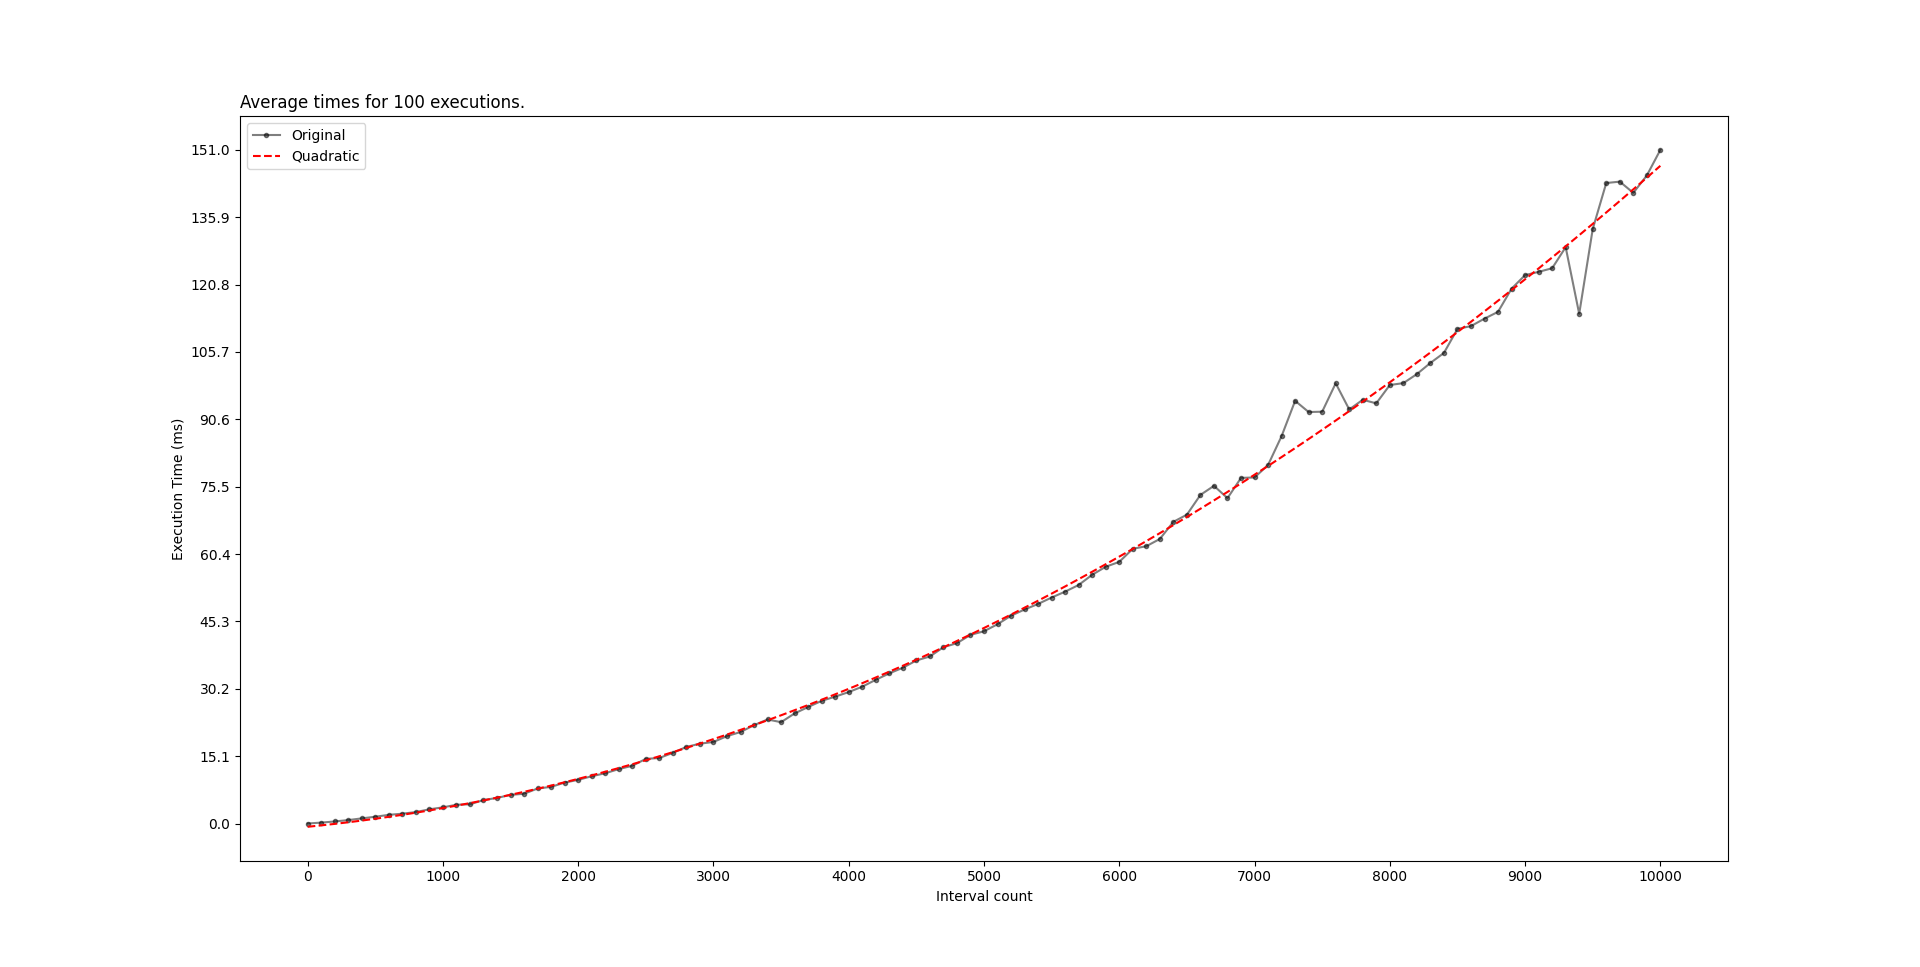
\includegraphics[width=1\textwidth]{../images/graphic_100Intervals.png}
    Este gráfico muestra el tiempo de ejecución promedio de 100 ejecuciones del programa (en milisegundos) dada una cantidad de intervalos con un acomodo cuadrático
\end{figure}

\begin{figure}[H]
	\centering
	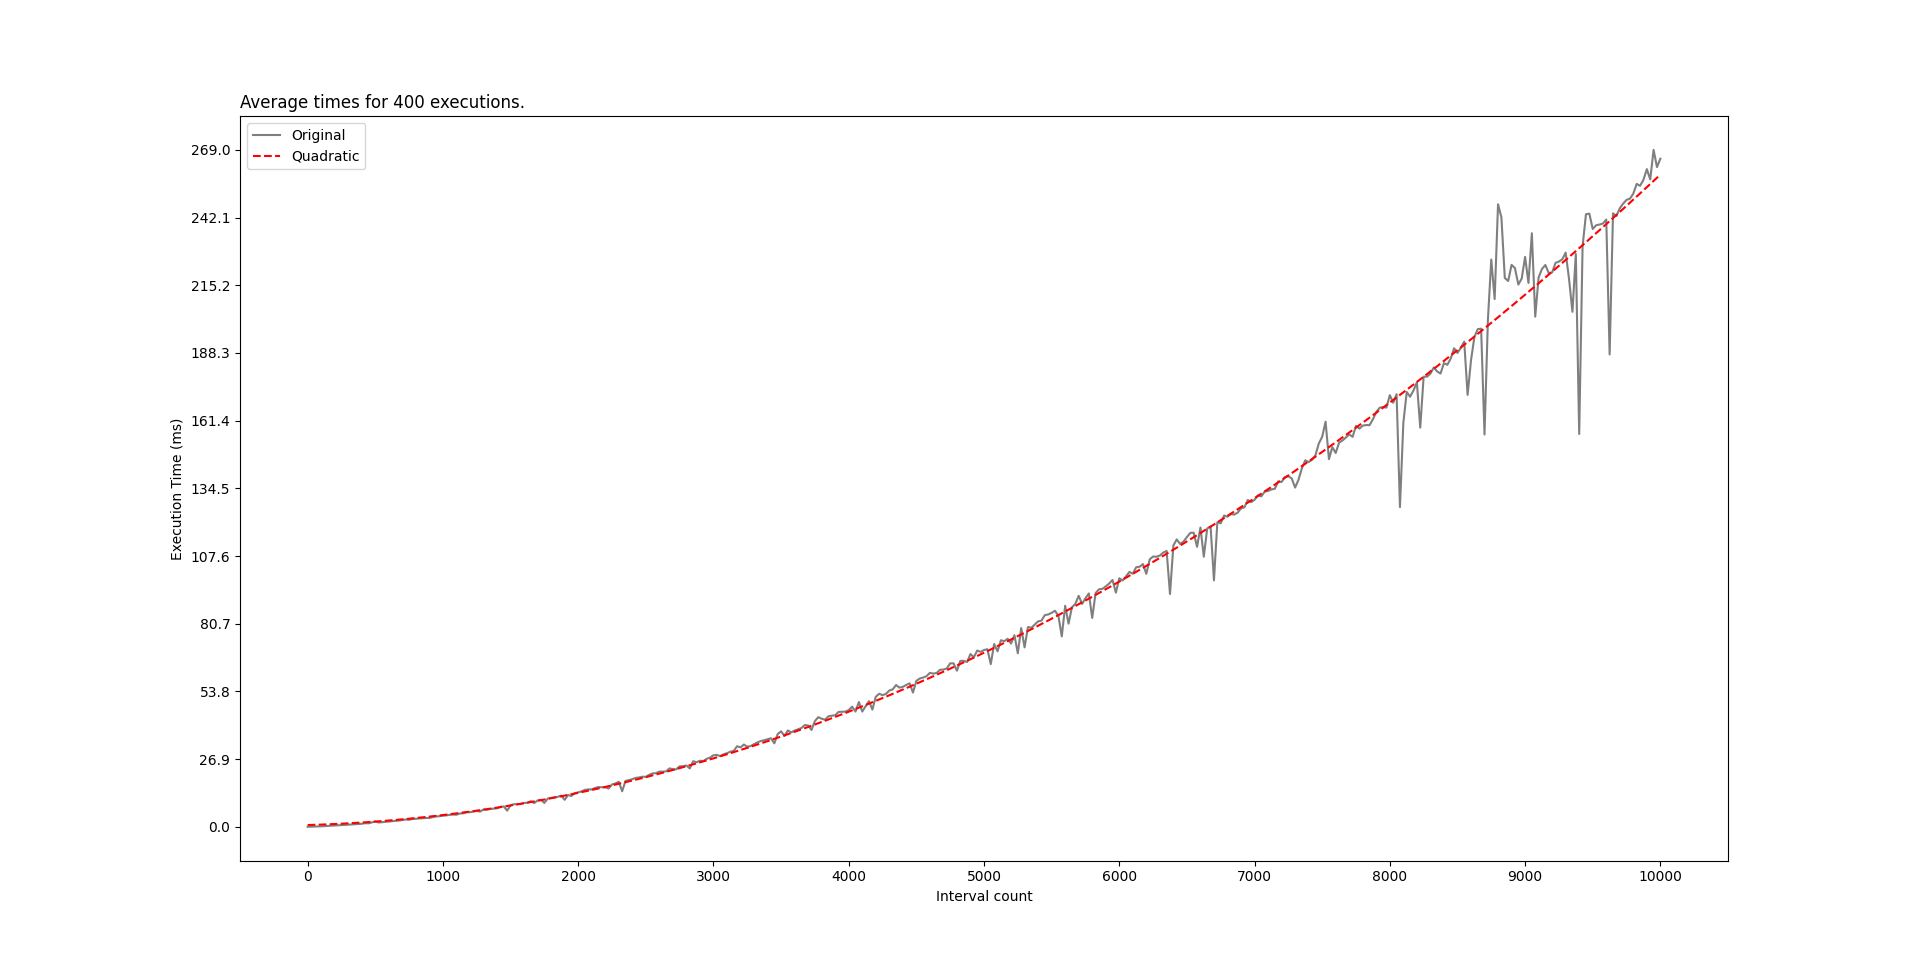
\includegraphics[width=1\textwidth]{../images/graphic_400Intervals.png}
	Este gráfico en cambio muestra el tiempo de ejecución pero del promedio de 400 ejecuciones del programa (en milisegundos)
\end{figure}

Como se puede apreciar, el gráfico muestra una tendencia cuadrática como lo explicado en el análisis de complejidad

\section{Conclusiones}

Acá irían las conclusiones de todo nuestro trabajo :)
}


\newpage
\end{document}